\documentclass{beamer}
\setbeamertemplate{bibliography item}{}
\usepackage[utf8]{vietnam}
\usepackage{graphicx}
\usepackage{booktabs}
\setbeamertemplate{bibliography item}[book]
\usetheme{Warsaw}
\newtheorem{dn}{Định nghĩa}[section]
\newtheorem{dl}{Định lý}[section]
\newtheorem{tc}{Tính chất}[section]
\newtheorem{hq}{Hệ quả}[section]
\newtheorem{bd}{Bổ đề}[section]
\newtheorem{md}{Mệnh đề}[section]
\newtheorem{vd}{Ví dụ}[section]
\newtheorem{nx}{Nhận xét}[section]
\newcommand{\dom}{\text{{\rm dom}}}
\newcommand{\epi}{\text{{\rm epi}}}
\newcommand{\Min}{\text{{\rm Min}}}
\setbeamertemplate{theorems}[numbered]
\setbeamertemplate{definitions}[numbered]
\setbeamertemplate{footline}[frame number]
\usepackage{algorithm}
\usepackage{color}
\usepackage{algorithmic}
\usepackage{footmisc}
%\usepackage{enumitem}
\usepackage{indentfirst} 
\usepackage{comment}
\renewcommand{\thefootnote}{\arabic{footnote}}
\usefonttheme{professionalfonts}
\setbeamercolor{normal text}{bg=white,fg=black}
\renewcommand{\thefootnote}{\arabic{footnote}}
%kt
\mode<presentation>
{
 \usetheme{Darmstadt}
%\usetheme{Rochester}
}
\beamertemplatetransparentcoveredhigh

\begin{document}
\title[]{\fontsize{13pt}{10pt}\selectfont {\bf \LARGE   Phương pháp giải bài toán \\Tối ưu tuyến tính nguyên}\\
------------------------------------------

{\small Hướng dẫn: PGS.TS. Tạ Quang Sơn}} 
\author[]{\bf Thực hiện : ĐỖ NGỌC MINH THƯ \& NGUYỄN CHÍ BẰNG \\
Sinh viên lớp: DTU1221, Khóa: 22}
\institute[Báo cáo luận văn thạc sĩ]{\fontsize{2pt}{2pt}}%
\small{\date{\today}}
\begin{frame}
\begin{center}
{\fontsize{8pt}{8pt}\selectfont \bf{ỦY BAN NHÂN DÂN THÀNH PHỐ HỒ CHÍ MINH\\
TRƯỜNG ĐẠI HỌC SÀI GÒN}}
\end{center}
\begin{center}
\end{center}

\begin{center}
{\fontsize{10pt}{6pt}\selectfont \bf{BÁO CÁO ĐỀ CƯƠNG NGHIÊN CỨU KHOA HỌC\\
NGÀNH: TOÁN ỨNG DỤNG}}
\end{center}
\titlepage
\end{frame}
\begin{frame}
    \frametitle{NỘI DUNG BÁO CÁO}
    \tableofcontents
\end{frame}

\section{Mục đích nghiên cứu}

\begin{frame}{Mục đích nghiên cứu}
    Tối ưu tuyến tính là một nội dung quan trọng trong chương trình đào tạo Cử nhân Toán ứng dụng. Lý thuyết về việc giải bài toán tối ưu tuyến tính đã được cung cấp cho sinh viên. Tuy vậy, có nhiều bài toán tối ưu cần được giải với nghiệm nguyên. Chẳng hạn như:
    \begin{itemize}
    \item Bài toán tối ưu nhân lực.
    \item Bài toán tối ưu vận chuyển hàng hóa.
    \item Bài toán tối ưu áp dụng trong tin học.
    \end{itemize}
\end{frame}
%bo
\begin{frame}{Ví dụ}
    Một công ty cần sản xuất 2 dòng xe máy để đưa ra thị trường. Biết rằng:
    \begin{itemize}
    \item Đối với dòng xe thứ nhất cần 2 \$ cho phụ tùng và 1 \$ cho chi phí thuê nhân công.
    \item Đối với dòng xe thứ hai cần 1 \$ cho phụ tùng và 3 \$ cho chi phí thuê nhân công.
    \item Tổng vốn đầu tư của công ty sẽ bỏ ra theo kế hoạch là 8 \$ cho phụ tùng và 10 \$ cho nhân công.
    \item Lợi nhuận của dòng xe thứ nhất là 2 \$ 1 sản phẩm và dòng thứ hai là 2 \$.
    \end{itemize}    
    Hãy tìm ra phương án đầu tư để đạt được lợi nhuận cao nhất.
\end{frame}
%bo
\begin{frame}{Ví dụ}
    \begin{center}                    
        \big(P\big)\quad $f(x)=2x_1+2x_2\quad \longrightarrow Max$\\
        \[\left\{\begin{aligned}
            &2x_1+x_2 \leq  8 \\
            &x_1+3x_2 \leq 10 \\
            &x_i\geq 0,\forall i=1,2
        \end{aligned}\right.\]\\
        \end{center}  
        Ta nhận được nghiệm $x_1=2.8$, $x_2=2.4$ và lợi nhuận nhận được là $10.4$.    
  
\end{frame}

\begin{frame}{Ví dụ}
    \begin{center}
        \begin{figure}[ht]
            \begin{center}

            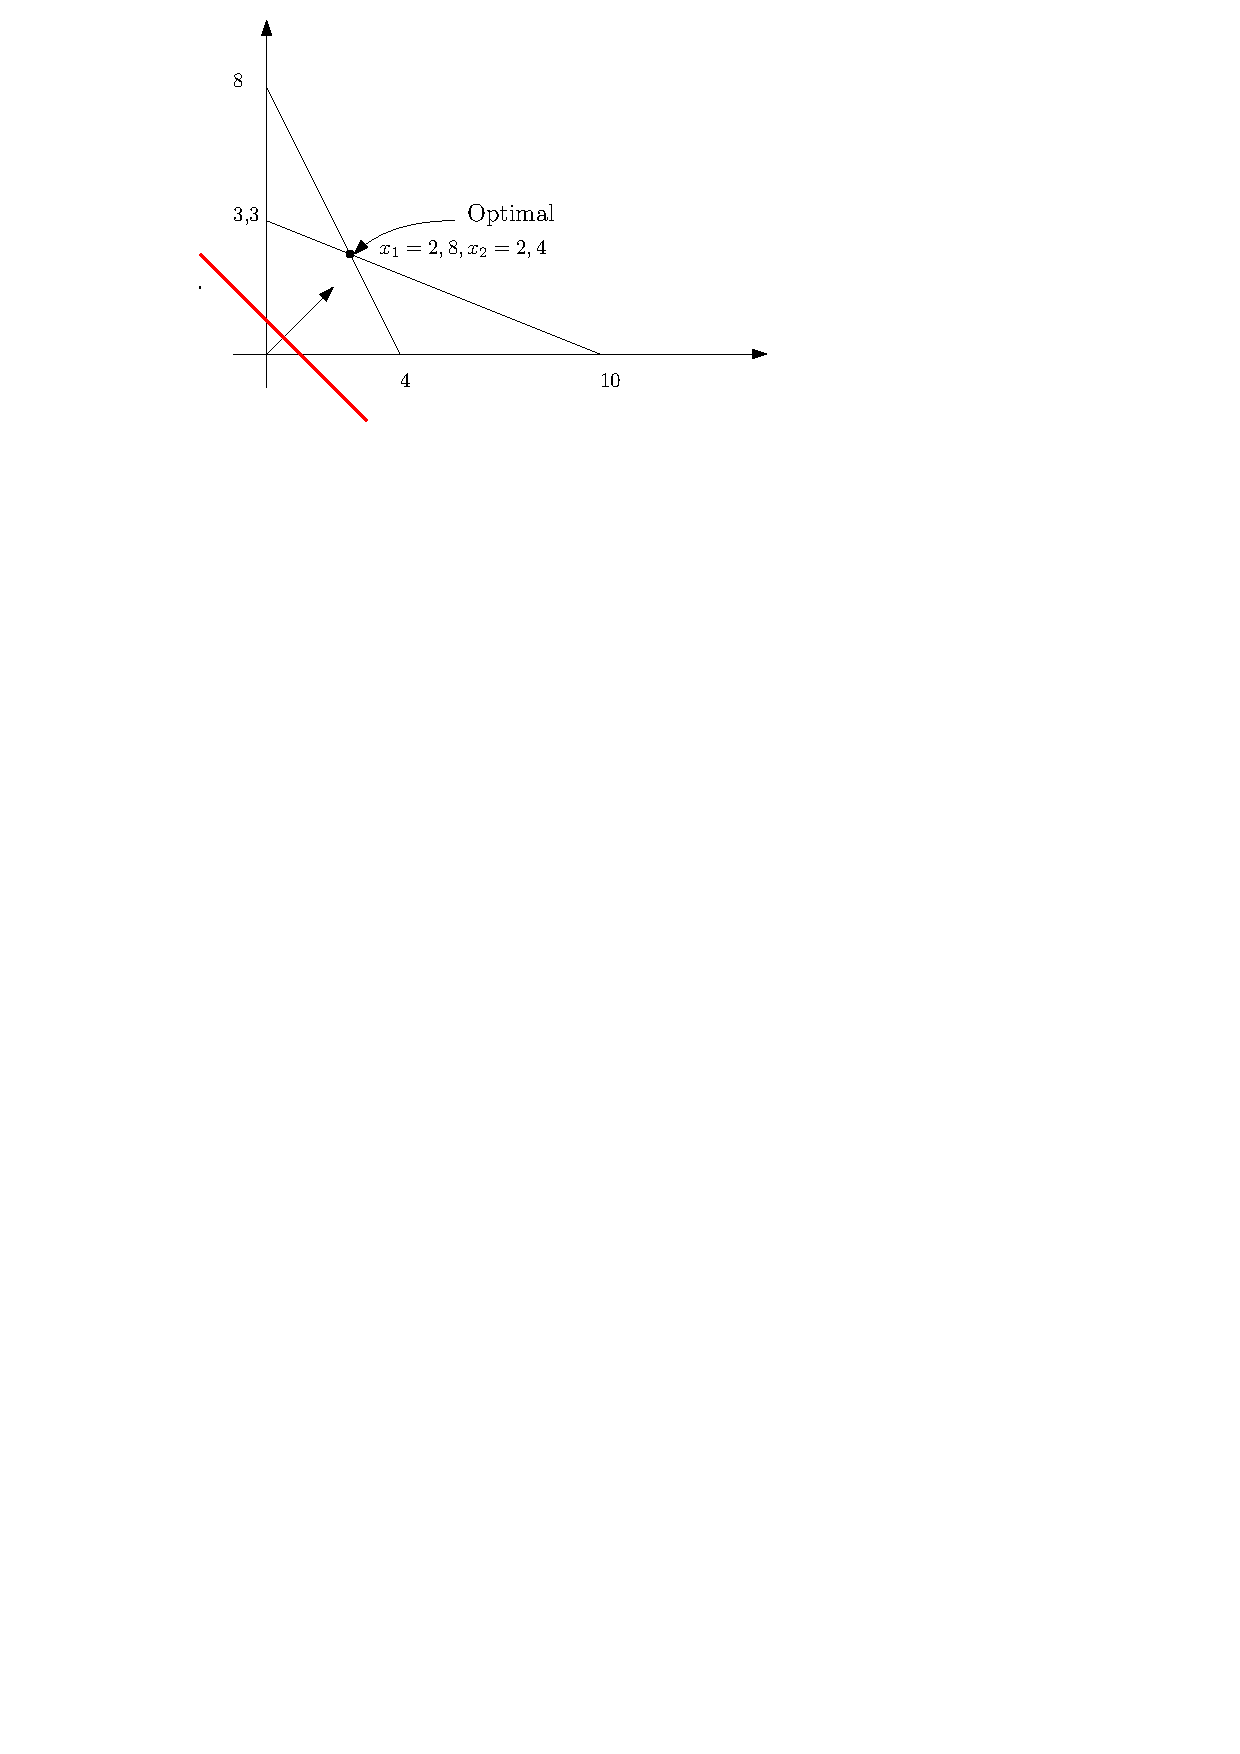
\includegraphics[width=0.7\linewidth]{/Users/chibangnguyen/Documents/GitHub/NCKH/BAOCAO/Nhom1_hinh.pdf}
            
            Hình minh hoạ bài toán
            \end{center}
      \end{figure}
      \end{center}
\end{frame}
\section{Nội dung nghiên cứu}
\begin{frame}{Nội dung nghiên cứu}
    \begin{itemize}
    \item Hệ thống lại cơ sở lý thuyết và phương pháp giải các bài toán Quy hoạch tuyến tính.
    \item Từ đó mở rộng để tìm nghiệm nguyên cho bài toán tối ưu nguyên, thông qua 2 phương pháp:
    \begin{itemize}
    \item Phương pháp Gomory.
    \item Phương pháp Land-Doig.
    \end{itemize}
    \end{itemize}
\end{frame}
\section{Dự kiến nội dung đề tài}
\begin{frame}{Dự kiến nội dung đề tài}
    \begin{itemize}
    \item Chương 1:  Bao gồm các kiến thức chuẩn bị, nội dung có liên quan đến
    một số kiến thức cơ bản của quy hoạch tuyến tính để dùng
    làm cơ sở nghiên cứu về các phương pháp giải của bài toán quy hoạch nguyên.
    \item Chương 2: Tìm hiểu về các phương pháp và thuật giải giúp giải quyết bài toán quy hoạch nguyên bằng phương pháp Gomory và phương pháp Land-Doig.
    \item Chương 3: Một số áp dụng của bài toán tối ưu nguyên vào các bài toán cụ thể trong kinh tế và khoa học.
    \end{itemize}   
\end{frame}
\section{Tổ chức và phân công}
\begin{frame}[shrink=20]
    \frametitle{Tổ chức và phân công}
    \vspace{1.5cm}
    \begin{table}
        \begin{tabular}{|c|c|c|}
            \hline
            Nội dung & Người phụ trách chính & Người cộng tác \\
            \hline \hline
            \textbf{Chương 1} && \\
            \hline
            Cơ sở lý thuyết quy hoạch tuyến tính & Đỗ Ngọc Minh Thư & \\
            & Nguyễn Chí Bằng & \\
            \hline
            \textbf{Chương 2} && \\
            \hline
            Phương pháp Gomory & Đỗ Ngọc Minh Thư & Nguyễn Chí Bằng \\
            Phương pháp Land-Doig & Nguyễn Chí Bằng & Đỗ Ngọc Minh Thư \\
            \hline
            \textbf{Chương 3} && \\
            \hline
            Một số áp dụng vào các bài
            toán cụ thể & Đỗ Ngọc Minh Thư & \\
            & Nguyễn Chí Bằng & \\
            \hline
        \end{tabular}
    \end{table}
\end{frame}
\section{Tiến độ thực hiện}
\begin{frame}{Tiến độ thực hiện}
Thời gian nghiên cứu chia làm 3 giai đoạn:
\begin{itemize}
\item Giai đoạn 1 (? tháng): Đọc, hiểu tài liệu liên quan đến lý thuyết tối ưu tuyến tính nguyên và các phương pháp giải.
\item Giai đoạn 2 (? tháng): Thu hoạch, hệ thống lại các tri thức và viết luận văn.
\item Giai đoạn 3 (? tháng): Hoàn thành và bảo vệ luận văn.
\end{itemize}
\end{frame}
\section{Tài liệu dùng cho nghiên cứu}
\begin{frame}[allowframebreaks]{Tài liệu dùng cho nghiên cứu}
    \scriptsize
    \begin{thebibliography}{}
        \bibitem{paper1} Tạ Quang Sơn, \textit{Bài giảng Quy hoạch tuyến tính}, Đại học Sài Gòn, 2023.
        \bibitem{paper2} Bùi Thế Tâm, \textit{Quy hoạch rời rạc}, Hà Nội, 10-2008.
        \bibitem{paper3} Michele Conforti, Gerard Cornuejols, and Giacomo Zambelli. \textit{Integer Programming}. Springer Publishing Company, Incorporated, 2014.
        \bibitem{paper4} G.B. Dantzig and M.N. Thapa. \textit{Linear Programming 2: 2: Theory and Extensions}. Linear Programming. Springer, 1997.
        \bibitem{paper5} George B. Dantzig and Mukund Narain Thapa. \textit{Linear Programming 1: Introduction}. Springer Series in Operations Research and Financial Engineering. Springer, New York, 1997.
        \bibitem{paper6} Ailsa H Land and Alison G Doig. \textit{An automatic method for solving discrete programming problems}. Springer, 2010.
        scriptsize
        \bibitem{paper7} GOMORY, R. E.: \textit{"Outline of an Algorithm for Integer Solutions to Linear Programs,"} Bulletin of the American Mathematical Society, 64, (1958), pp. 275-8.
    \end{thebibliography}
\end{frame}
\end{document}
